%% Aetherion architecture diagram for the JOSS paper.
%% Build:  pdflatex architecture && pdftoppm -png -r 300 -singlefile architecture.pdf architecture
%% Only architecture.png is tracked (*.pdf is gitignored repo-wide).
%% JOSS-only figure: do not reuse it in the AST paper; draw a new one there.
\documentclass[border=3pt]{standalone}
\usepackage[T1]{fontenc}
\usepackage{lmodern}
\usepackage[scaled=0.92]{helvet}
\renewcommand{\familydefault}{\sfdefault}
\usepackage{amsmath,amssymb}
\usepackage{tikz}
\usetikzlibrary{arrows.meta,calc}

\newcommand{\code}[1]{\texttt{#1}}

%% \layer{x}{y}{w}{h}{label}: a shaded layer frame, top-left at (x,y), in mm
\newcommand{\layer}[5]{%
  \draw[draw=black!35, fill=black!4, rounded corners=3pt] (#1,#2) rectangle ++(#3,-#4);
  \node[anchor=north west, font=\scriptsize\bfseries, text=black!60, inner sep=1.2pt]
    at (#1+0.6,#2-0.4) {#5};}

\begin{document}
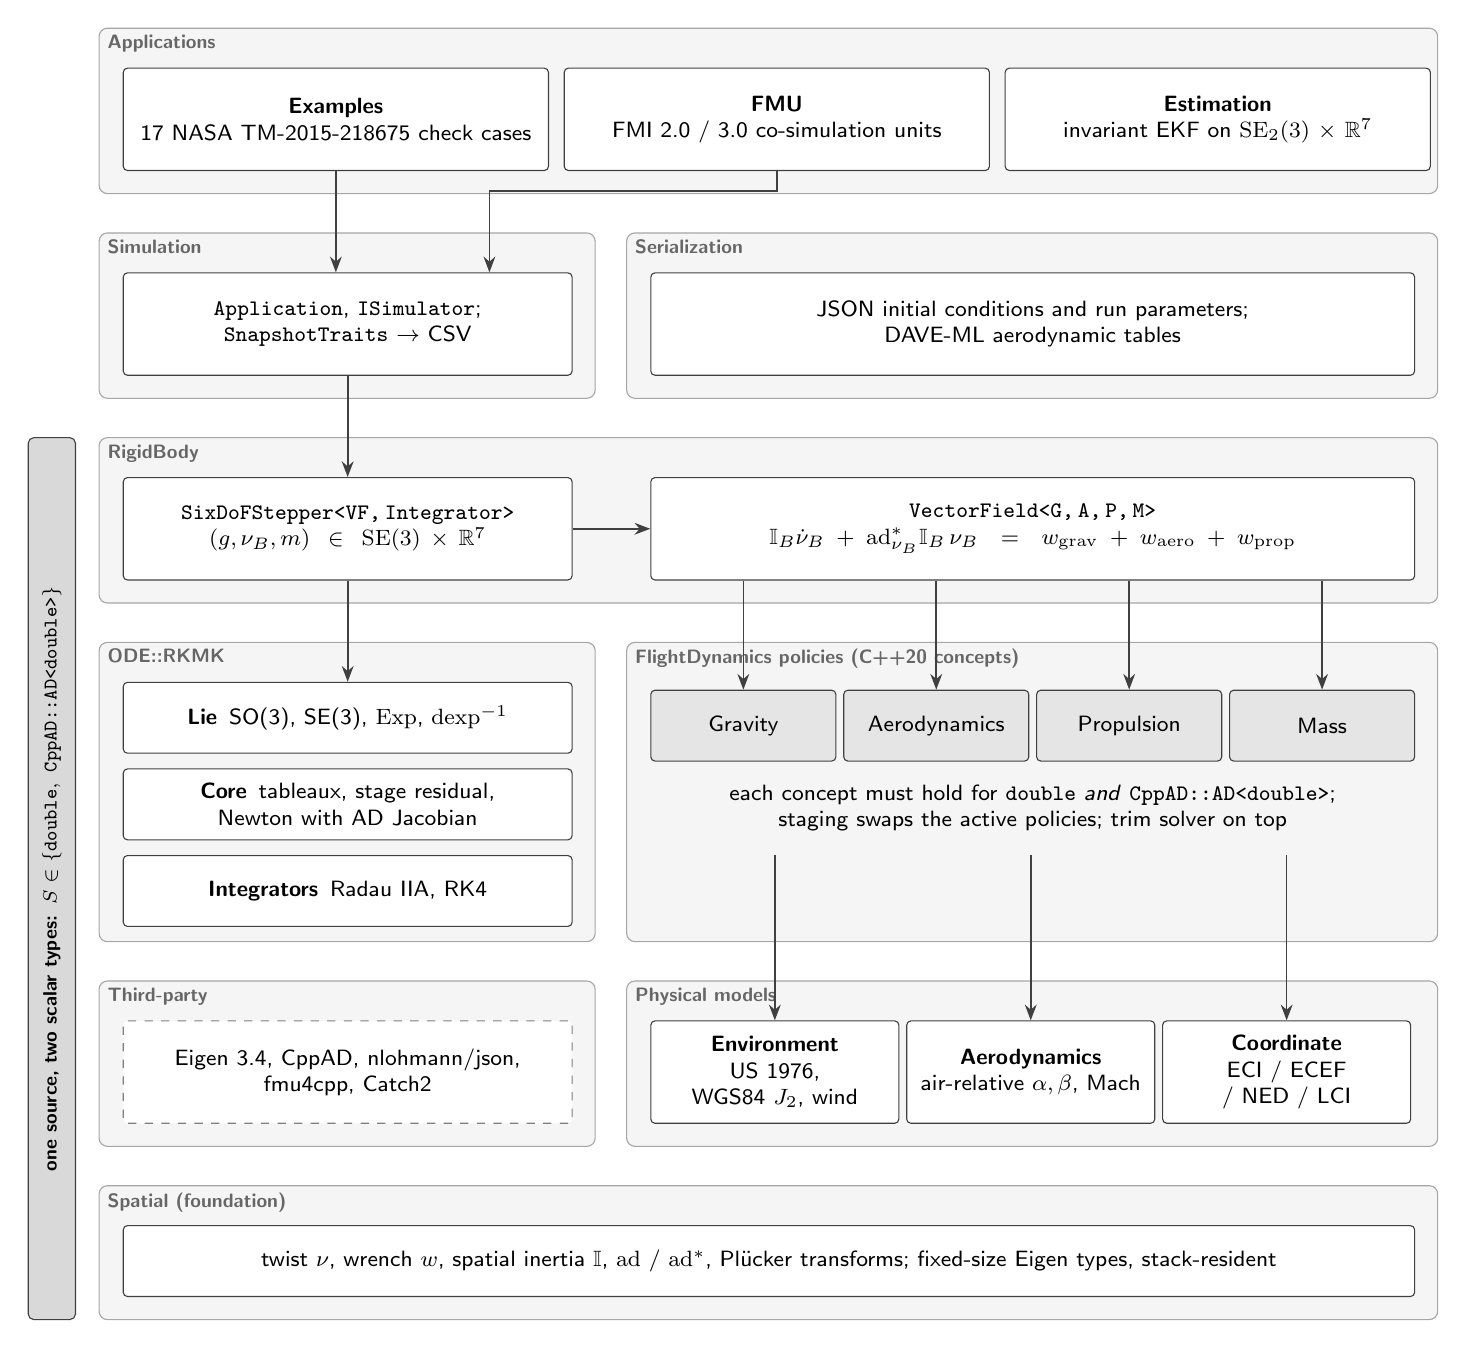
\begin{tikzpicture}[
    x=1mm, y=1mm,
    font=\footnotesize,
    box/.style 2 args={draw=black!75, fill=white, rounded corners=1.5pt,
                       anchor=north west, align=center, inner sep=1.5pt,
                       text width=#1 mm - 3pt, minimum height=#2 mm},
    pol/.style={box={#1}{9}, fill=black!10},
    use/.style={-{Stealth[length=2mm]}, semithick, black!75},
  ]

  %% Left column x = 0..63, right column x = 67..170.

  %% --- Applications ---------------------------------------------------------
  \layer{0}{0}{170}{21}{Applications}
  \node[box={54}{13}] (ex)  at (3,-5)   {\textbf{Examples}\\17 NASA TM-2015-218675 check cases};
  \node[box={54}{13}] (fmu) at (59,-5)  {\textbf{FMU}\\FMI 2.0 / 3.0 co-simulation units};
  \node[box={54}{13}] (est) at (115,-5) {\textbf{Estimation}\\invariant EKF on
                                         $\mathrm{SE}_2(3)\times\mathbb{R}^7$};

  %% --- Driver and I/O -------------------------------------------------------
  \layer{0}{-26}{63}{21}{Simulation}
  \node[box={57}{13}] (sim) at (3,-31)
       {\code{Application}, \code{ISimulator};\\\code{SnapshotTraits} $\to$ CSV};
  \layer{67}{-26}{103}{21}{Serialization}
  \node[box={97}{13}] (ser) at (70,-31)
       {JSON initial conditions and run parameters;\\DAVE-ML aerodynamic tables};

  %% --- RigidBody ------------------------------------------------------------
  \layer{0}{-52}{170}{21}{RigidBody}
  \node[box={57}{13}] (step) at (3,-57)
       {\code{SixDoFStepper<VF,\,Integrator>}\\
        $(g,\nu_B,m)\in\mathrm{SE}(3)\times\mathbb{R}^{7}$};
  \node[box={97}{13}] (vf) at (70,-57)
       {\code{VectorField<G,\,A,\,P,\,M>}\\
        $\mathbb{I}_B\dot{\nu}_B+\mathrm{ad}^{*}_{\nu_B}\mathbb{I}_B\,\nu_B
         = w_{\mathrm{grav}}+w_{\mathrm{aero}}+w_{\mathrm{prop}}$};

  %% --- ODE::RKMK and FlightDynamics policies --------------------------------
  \layer{0}{-78}{63}{38}{ODE::RKMK}
  \node[box={57}{9}] (lie)  at (3,-83)   {\textbf{Lie}\enspace SO(3), SE(3), $\mathrm{Exp}$, $\mathrm{dexp}^{-1}$};
  \node[box={57}{9}] (core) at (3,-94)   {\textbf{Core}\enspace tableaux, stage residual,\\Newton with AD Jacobian};
  \node[box={57}{9}] (int)  at (3,-105)  {\textbf{Integrators}\enspace Radau IIA, RK4};

  \layer{67}{-78}{103}{38}{FlightDynamics policies (C++20 concepts)}
  \node[pol={23.5}] (pg) at (70,-84)    {Gravity};
  \node[pol={23.5}] (pa) at (94.5,-84)  {Aerodynamics};
  \node[pol={23.5}] (pp) at (119,-84)   {Propulsion};
  \node[pol={23.5}] (pm) at (143.5,-84) {Mass};
  \node[anchor=north west, text width=97mm, align=center, inner sep=0pt] at (70,-96)
       {each concept must hold for \code{double} \emph{and}
        \code{CppAD::AD<double>};\\ staging swaps the active policies;
        trim solver on top};

  %% --- Physical models and third-party --------------------------------------
  \layer{0}{-121}{63}{21}{Third-party}
  \node[box={57}{13}, draw=black!50, dashed] (dep) at (3,-126)
       {Eigen 3.4, CppAD, nlohmann/json,\\fmu4cpp, Catch2};
  \layer{67}{-121}{103}{21}{Physical models}
  \node[box={31.5}{13}] (env)   at (70,-126)  {\textbf{Environment}\\US 1976, WGS84 $J_2$, wind};
  \node[box={31.5}{13}] (aero)  at (102.5,-126) {\textbf{Aerodynamics}\\air-relative $\alpha,\beta$, Mach};
  \node[box={31.5}{13}] (coord) at (135,-126) {\textbf{Coordinate}\\ECI / ECEF / NED / LCI};

  %% --- Spatial --------------------------------------------------------------
  \layer{0}{-147}{170}{17}{Spatial (foundation)}
  \node[box={164}{9}] (spa) at (3,-152)
       {twist $\nu$, wrench $w$, spatial inertia $\mathbb{I}$, $\mathrm{ad}$ / $\mathrm{ad}^{*}$,
        Pl\"ucker transforms; fixed-size Eigen types, stack-resident};

  %% --- Scalar-type band -----------------------------------------------------
  \draw[draw=black!75, fill=black!15, rounded corners=2pt] (-9,-52) rectangle (-3,-164);
  \node[rotate=90, font=\scriptsize\bfseries] at (-6,-108)
       {one source, two scalar types:\enspace
        $S\in\{\code{double},\ \code{CppAD::AD<double>}\}$};

  %% --- Uses arrows (user $\to$ used) ----------------------------------------
  \draw[use] (ex.south)  -- (ex.south |- sim.north);
  \draw[use] (fmu.south) -- ++(0,-2.5) -| ([xshift=18mm]sim.north);
  \draw[use] (sim.south) -- (step.north);
  \draw[use] (step.east) -- (vf.west);
  \draw[use] (step.south) -- (lie.north);
  \foreach \p in {pg,pa,pp,pm}
    \draw[use] (vf.south -| \p.north) -- (\p.north);
  \foreach \m in {env,aero,coord}
    \draw[use] (\m.north |- 0,-105) -- (\m.north);
\end{tikzpicture}
\end{document}
